\title{The title of the paper}
\author{
        Philippe de~Groote \\
                INRIA
            \and
       Ekaterina Lebedeva\\
        INRIA
}
\date{\today}

\documentclass[a4paper,12pt]{article}

\usepackage{amsmath}
\usepackage{amsthm}
\usepackage{amssymb}
\usepackage{stmaryrd}
\usepackage{mathrsfs,cmll}
\usepackage[sans]{dsfont}
\usepackage{graphicx}

\usepackage{lingmacros} % linguistic macros for enumerating sentences

% Dynamic connectives and quantifiers

\newcommand{\dynexists}{\mathord{\reflectbox{$\mathds{E}$}}}

\newcommand{\dynall}{\mathord{%
\raisebox{\depth}{\rotatebox{180}{$\mathds{A}$}}}}

\newcommand{\dynor}{\mathbin{\mathds{V}}}

\newcommand{\dynand}{\mathbin{%
\reflectbox{\raisebox{\depth}{\rotatebox{180}{${\dynor}$}}}}}

\newcommand{\dynimplies}{\mathbin{%
\mbox{\raisebox{.28ex}{\rule{1.7ex}{.15ex}}%
\hspace{-1.7ex}\raisebox{.73ex}{\rule{1.7ex}{.15ex}}%
\hspace{-.4ex}\raisebox{-.01ex}{\rotatebox{45}{\rule{.83ex}{.15ex}}}%
\hspace{-.69ex}\raisebox{.58ex}{\rotatebox{135}{\rule{.83ex}{.15ex}}}}
}}

\newcommand{\dynneg}{\mathop{%
\mbox{\raisebox{.68ex}{\rule{1.2ex}{.15ex}}%
\hspace{-.15ex}\raisebox{.2ex}{\rule{.15ex}{.63ex}}%
\hspace{.25ex}\raisebox{.2ex}{\rule{.15ex}{.63ex}}\hspace{.15ex}}
}}

%%%%% lambda-terms

\newif\ifatomic
\newif\ifoperator
\newif\ifconj
\newif\ifdisj
\newif\ifdconj
\newif\ifddisj

\def\reset{\atomicfalse\operatorfalse\conjfalse\disjfalse\dconjfalse\ddisjfalse}

% abstraction

\def\abs#1#2%
{\ifatomic%
(\lambda #1 . \, \reset #2)%
\else%
\lambda #1 . \, \reset #2%
\fi\reset}

% application

\def\app#1#2%
{\ifoperator%
\reset\atomictrue\operatortrue #1 \, \reset\atomictrue #2%
\else%
\ifatomic%
(\reset\atomictrue\operatortrue #1 \, \reset\atomictrue #2)%
\else%
\reset\atomictrue\operatortrue #1 \, \reset\atomictrue #2%
\fi%
\fi\reset}

% universal quantification

\def\uquant#1#2%
{\ifatomic%
(\forall #1 . \, \reset #2)%
\else%
\forall #1 . \, \reset #2%
\fi\reset}

% existential quantification

\def\equant#1#2%
{\ifatomic%
(\exists #1 . \, \reset #2)%
\else%
\exists #1 . \, \reset #2%
\fi\reset}

% implication

\def\imp#1#2%
{\ifatomic%
(\reset\atomictrue #1 \rightarrow \reset\atomictrue #2)%
\else%
\reset\atomictrue #1 \rightarrow \reset\atomictrue #2%
\fi\reset}

% conjunction

\def\conj#1#2%
{\ifconj%
\reset\atomictrue\conjtrue #1 \wedge \reset\atomictrue\conjtrue #2%
\else%
\ifatomic%
(\reset\atomictrue\conjtrue #1 \wedge \reset\atomictrue\conjtrue #2)%
\else%
\reset\atomictrue\conjtrue #1 \wedge \reset\atomictrue\conjtrue #2%
\fi%
\fi\reset}

% disjunction

\def\disj#1#2%
{\ifdisj%
\reset\atomictrue\disjtrue #1 \vee \reset\atomictrue\disjtrue #2%
\else%
\ifatomic%
(\reset\atomictrue\disjtrue #1 \vee \reset\atomictrue\disjtrue #2)%
\else%
\reset\atomictrue\disjtrue #1 \vee \reset\atomictrue\disjtrue #2%
\fi%
\fi\reset}

% negation

\def\nega#1%
{\neg \reset\atomictrue #1\reset}

% dynamic universal quantification

\def\duquant#1#2%
{\ifatomic%
(\dynall #1 . \, \reset #2)%
\else%
\dynall #1 . \, \reset #2%
\fi\reset}

% dynamic existential quantification

\def\dequant#1#2%
{\ifatomic%
(\dynexists #1 . \, \reset #2)%
\else%
\dynexists #1 . \, \reset #2%
\fi\reset}

% dynamic implication

\def\dimp#1#2%
{\ifatomic%
(\reset\atomictrue #1 \dynimplies \reset\atomictrue #2)%
\else%
\reset\atomictrue #1 \dynimplies \reset\atomictrue #2%
\fi\reset}

% dynamic conjunction

\def\dconj#1#2%
{\ifdconj%
\reset\atomictrue\dconjtrue #1 \dynand \reset\atomictrue\dconjtrue #2%
\else%
\ifatomic%
(\reset\atomictrue\dconjtrue #1 \dynand \reset\atomictrue\dconjtrue #2)%
\else%
\reset\atomictrue\dconjtrue #1 \dynand \reset\atomictrue\dconjtrue #2%
\fi%
\fi\reset}

% dynamic disjunction

\def\ddisj#1#2%
{\ifddisj%
\reset\atomictrue\ddisjtrue #1 \dynor \reset\atomictrue\ddisjtrue #2%
\else%
\ifatomic%
(\reset\atomictrue\ddisjtrue #1 \dynor \reset\atomictrue\ddisjtrue #2)%
\else%
\reset\atomictrue\ddisjtrue #1 \dynor \reset\atomictrue\ddisjtrue #2%
\fi%
\fi\reset}

% dynamic negation

\def\dnega#1%
{\dynneg \reset\atomictrue #1\reset}

%%%%%%%%%%%%%%%%%%%%%%%%


%------------------------------------------------------------------------------------
\newcommand{\existsA}{\exists}
\newcommand{\existsB}{\dynexists} 

\newcommand{\forallA}{\exists}
\newcommand{\forallB}{\dynall}  

\newcommand{\impA}{\rightarrow}
\newcommand{\impB}{\dynimplies}

\newcommand{\negA}{\neg}
\newcommand{\negB}{\dynneg}

\newcommand{\landA}{\land}
\newcommand{\landB}{\dynand}

\newcommand{\lorA}{\lor}
\newcommand{\lorB}{\dynor} 


%------------------------------------------------------------------------------------
% New Commands: Miscelaneous abbreviations
%------------------------------------------------------------------------------------

\newcommand{\I}[1]{[\![#1]\!]}  % interpretation

\newcommand{\txt}[1]{\textit{#1}} % italic
\newcommand{\defeq}{\doteq} % equal by definition
\newcommand{\logeq}{\equiv} % logical equivalence
\newcommand{\seq}{=_s} % syntactic equality
\newcommand{\nseq}{\neq_s} % syntactic non-equality

\newcommand{\congr}{=_{\alpha}} % alpha-congruent
\newcommand{\ncongr}{\neq_{\alpha}} % alpha non-congruent



\newcommand{\trr}[1]{#1} % this one does not do anything

\newcommand{\Types}{\text{T}} % Types


\newcommand{\upii}[2]{#1 ::  #2}  % list constructor
\newcommand{\sel}{\mathsf{sel} } % selection function
\newcommand{\updt}{\mathsf{upd}}  % discourse update
\newcommand{\D}{\mathbf{D}} % discourse
\renewcommand{\S}{\mathbf{S}} % sentence

\newcommand{\tr}[1]{\overline{#1}} % dynamizing
\newcommand{\ttr}[1]{ \overline{#1}^*} 
\newcommand{\etr}[1]{ \widetilde{#1}} % non-conventional dynamic term

%------------------------------------------------------------------------------------
% New Commands: Lambda Calculus
%------------------------------------------------------------------------------------
\newcommand{\bconv}{\rightarrow_\beta}  %one-step beta reduction
\newcommand{\bred}{\rightarrow^{*}_\beta} %beta reduction
\newcommand{\econv}{\rightarrow_\eta} %eta conversion 


%------------------------------------------------------------------------------------
% New Commands: 
% Abbreviations for distinguishing variables for static and dynamic cases.
% E.g.: \x1 - static, \x2 - dynamic
%------------------------------------------------------------------------------------
\newcommand{\A}[1]{\ifcase #1 \or \AAA\or\AB\or\AC\fi}
\newcommand{\B}[1]{\ifcase #1 \or \BA\or\BB\or\BC\fi}
\newcommand{\R}[1]{\ifcase #1 \or \RA\or\RB\or\RC\fi}
\newcommand{\Q}[1]{\ifcase #1 \or \QA\or\QB\or\QC\fi}
\renewcommand{\P}[1]{\ifcase #1 \or \PA\or\PB\or\PC\fi}
\newcommand{\X}[1]{\ifcase #1 \or \XA\or\XB\or\XC\fi}
\newcommand{\Y}[1]{\ifcase #1 \or \YA\or\YB\or\YC\fi}
\newcommand{\x}[1]{\ifcase #1 \or \xA\or\xB\or\xC\fi}
\newcommand{\y}[1]{\ifcase #1 \or \yA\or\yB\or\yC\fi}
\newcommand{\z}[1]{\ifcase #1 \or \zA\or\zB\or\zC\fi}
\renewcommand{\t}[1]{\ifcase #1 \or \tA\or\tB\or\tC\fi}
\newcommand{\h}[1]{\ifcase #1 \or \hA\or\hB\or\hC\fi}
\renewcommand{\v}[1]{\ifcase #1 \or \vA\or\vB\or\vC\fi}
\renewcommand{\u}[1]{\ifcase #1 \or \uA\or\uB\or\uC\fi}
\newcommand{\w}[1]{\ifcase #1 \or \wA\or\wB\or\wC\fi}

%------------------------------------------------------------------------------------

\newcommand{\AAA}{\mathrm{A}}
\newcommand{\AB}{\mathbf{A}}
\newcommand{\AC}{\varmathbb{A}}

\newcommand{\BA}{\mathrm{B}}
\newcommand{\BB}{\mathbf{B}}
\newcommand{\BC}{\varmathbb{B}}


\newcommand{\RA}{\mathrm{R}}
\newcommand{\RB}{\mathbf{R}}
\newcommand{\RC}{\varmathbb{R}}

\newcommand{\QA}{\mathrm{Q}}
\newcommand{\QB}{\mathbf{Q}}
\newcommand{\QC}{\varmathbb{Q}}

\newcommand{\PA}{\mathrm{P}}
\newcommand{\PB}{\mathbf{P}}
\newcommand{\PC}{\varmathbb{P}}

\newcommand{\XA}{\mathrm{X}}
\newcommand{\XB}{\mathbf{X}}
\newcommand{\XC}{\varmathbb{X}}

\newcommand{\YA}{\mathrm{Y}}
\newcommand{\YB}{\mathbf{Y}}
\newcommand{\YC}{\varmathbb{Y}}

\newcommand{\xA}{x}
\newcommand{\xB}{\mathbf{x}}
\newcommand{\xC}{\mathbf{x}}

\newcommand{\yA}{y}
\newcommand{\yB}{\mathbf{y}}
\newcommand{\yC}{\mathbf{y}}

\newcommand{\zA}{z}
\newcommand{\zB}{\mathbf{z}}
\newcommand{\zC}{\mathbf{z}}

\newcommand{\tA}{t}
\newcommand{\tB}{\mathbf{t}}
\newcommand{\tC}{\mathbf{t}}

\newcommand{\hA}{h}
\newcommand{\hB}{\mathbf{h}}
\newcommand{\hC}{\mathbf{h}}

\newcommand{\vA}{v}
\newcommand{\vB}{\mathbf{v}}
\newcommand{\vC}{\mathbf{v}}

\newcommand{\uA}{u}
\newcommand{\uB}{\mathbf{u}}
\newcommand{\uC}{\mathbf{u}}

\newcommand{\wA}{w}
\newcommand{\wB}{\mathbf{w}}
\newcommand{\wC}{\mathbf{w}}



%------------------------------------------------------------------------------------
% New Commands: Non-logical constants
%------------------------------------------------------------------------------------

\newcommand{\cfarmer}{\textbf{f} }
\newcommand{\cdonkey}{\textbf{d} }
\newcommand{\cown}{\textbf{o} }
\newcommand{\cbeat}{\textbf{b} }

%------------------------------------------------------------------------------------
% New Commands: Frameworks
%------------------------------------------------------------------------------------

\newcommand{\expn}{\chi}  % exception

\newcommand{\G}{G$_0$} % framework introduced in SALT 2006 paper
\newcommand{\GN}{G} % first order framework
\newcommand{\GL}{GL} % higher order framework
\newcommand{\GLex}{GL$\expn$} % dynamic logic with exceptions

\newcommand{\ex}[1]{\ifcase #1 \or \existsA\or\existsB\or\existsC\fi}
\newcommand{\all}[1]{\ifcase #1 \or \forallA\or\forallB\or\forallC\fi}
%\newcommand{\imp}[1]{\ifcase #1 \or \impA\or\impB\or\impC\fi}
\newcommand{\dsj}[1]{\ifcase #1 \or \lorA\or\lorB\or\lorC\fi}
\newcommand{\n}[1]{\ifcase #1 \or \negA\or\negB\or\negC\fi}
\newcommand{\cnj}[1]{\ifcase #1 \or \landA\or\landB\or\landC\fi}

%------------------------------------------------------------------------------------
% New Commands: Colorful symbols for the comparison with DPL
%------------------------------------------------------------------------------------



\newcommand{\ntodl}{h_G}
%\newcommand{trntog}{$h_g$}

\newcommand{\ntodpl}{h_{\textit{DPL}}}

\newcommand{\dpltos}{s_{DPL}}
\newcommand{\mdpltos}[1]{ ( #1 )_{s_\textit{DPL}}}

\newcommand{\dltos}{\textcolor{red}{s_{G}}}
\newcommand{\mdltos}[1]{ \textcolor{red}{(} #1 \textcolor{red}{)_{s_{G}}}}

\newcommand{\dplstodls}{\textcolor{blue}{\lceil \cdot \rceil_S}}
\newcommand{\mdplstodls}[1]{\textcolor{blue}{\lceil}  #1 \textcolor{blue}{\rceil_S}}

\newcommand{\dplstodpll}{\textcolor{cyan}{t^{\lambda}_\textit{DPL}}}
\newcommand{\mdplstodpll}[1]{\textcolor{cyan}{(} #1 \textcolor{cyan}{ )_{t^{\lambda}_\textit{DPL}}}}

\newcommand{\dpltodl}{\textcolor{cyan}{t^{G}_\textit{DPL}}}
\newcommand{\mdpltodl}[1]{\textcolor{cyan}{(} #1 \textcolor{cyan}{ )_{t^{G}_\textit{DPL}}}}


\newcommand{\dpllstodl}{\textcolor{blue}{\lceil \cdot \rceil_L}}
\newcommand{\mdpllstodl}[1]{\textcolor{blue}{\lceil} #1 \textcolor{blue}{\rceil_L}}

\newcommand{\newDPL}{\textit{DPL}^\lambda_L}

\newcommand{\statesDPL}{\textit{DPL}_{S}}
\newcommand{\statesDL}{\GN_S}

\newcommand{\langDPL}{\textit{DPL}_L}
\newcommand{\langDL}{\GN_L}



\newcommand{\qex}{\qed}
%
%       Italized theorem-like environments
%
\newtheorem{theorem}{Theorem}[section]
\newtheorem{conjecture}[theorem]{Conjecture}
\newtheorem{lemma}[theorem]{Lemma}
\newtheorem{proposition}[theorem]{Proposition}
\newtheorem{corollary}[theorem]{Corollary}
\newtheorem{principle}[theorem]{Principle}
%
%       Non-italized theorem-like environments:
%
\newtheorem{@definition}[theorem]{Definition}
\newenvironment{definition}{\begin{@definition}\upshape}{\end{@definition}}
\newtheorem{@remark}[theorem]{Remark}
\newenvironment{remark}{\begin{@remark}\upshape}{\end{@remark}}
\newtheorem{@notation}[theorem]{Notation}
\newenvironment{notation}{\begin{@notation}\upshape}{\end{@notation}}
\newtheorem{@example}[theorem]{Example}
\newenvironment{example}{\begin{@example}\upshape }{ \qex\end{@example}}
\newtheorem{@convention}[theorem]{Convention}
\newenvironment{convention}{\begin{@convention}\upshape}{\end{@convention}}
\newtheorem{@note}[theorem]{Note}
\newenvironment{note}{\begin{@note}\upshape}{\end{@note}}

\begin{document}
\maketitle

\begin{abstract}
This is the paper's abstract \ldots
\end{abstract}

\section{Introduction}
This is the paper's introduction.

\section{The Underlying Dynamic Logics}

Philippe de Groote~\cite{deGroote:2006:Towards-a-Montagovian-Account-of-Dynamics} showed that it is possible to handle dynamic phenomena of natural language by standard tools of mathematical logic, such as simply-typed lambda calculus, and, therefore, stay within Montague's program. This is accomplished in de~Groote's framework, called below {\G}, by providing Montague semantics with a notion of context in a systematic and precise way. 

The meaning of a sentence is a function of the context. It can be expressed in lambda calculus by defining the term standing for the interpretation of a sentence as an abstraction over a variable standing for the context. 

\begin{definition}[Context, Environment] A \textbf{context} or \textbf{environment} is a term of type $\gamma$ that stores the essential information from what has already been processed in the computation of the meaning of the whole discourse.
\end{definition}

In order to make the framework flexible, the context type $\gamma$ is a parameter, which can define any complex type. Therefore, there is no restriction on the representation of context. One can define it as a simple structure focusing on a particular phenomenon and elaborate it as more complex phenomena are considered.

A sentence can have a potential to change (or update) the context. The updated context has to be passed as an argument to the meaning of the subsequent sentence. In order to do so compositionally, de~Groote used the notion of continuation: the meaning of a sentence not only is a function of a context, but also is a function of a continuation with respect to the computation of the meaning of the whole discourse. Within the body of the term standing for the meaning of a sentence, the continuation is given the possibly updated context and returns a proposition. Therefore, the continuation has type $(\gamma \rightarrow o)$.
\begin{definition}[Continuation] A \textbf{continuation} is a term of type $(\gamma \rightarrow o)$ that denotes what is still to be processed in the computation of the meaning of the whole discourse. 
\end{definition}

Thus, a sentence is dynamically interpreted as a function that takes a context $e$ of type $\gamma$ and a continuation $\phi$ of type $(\gamma \rightarrow o)$ and returns a proposition: % i.e. the meaning of a sentence is a term of type $(\gamma \imp1 (\gamma \imp1 o) \imp1 o)$:
\begin{align}
\I{s} = \underbrace{\gamma}_{\text{context}} \rightarrow \underbrace{(\gamma \rightarrow o)}_{\text{continuation}} \rightarrow \underbrace{o}_{
\text{proposition}} \notag
\end{align}
Type $(\gamma \rightarrow (\gamma \rightarrow o) \rightarrow o)$ is, therefore, defined to be the type of a dynamic proposition.
 
\begin{example} \label{ex:2006-jlm} The meaning of the sentence~\eqref{sent:JlovesM-2006} is the $\lambda$-term~\eqref{eq:ex:lovejm}:
\enumsentence{ \txt{John loves Mary.} \label{sent:JlovesM-2006}}
\begin{align}
\underbrace{\lambda \overbrace{\underbrace{e^{\gamma}}_{\text{context}} \underbrace{\phi^{\gamma \rightarrow o}}_{\text{continuation}}.  \overbrace{\overbrace{ \overbrace{\textbf{love}^{\iota \rightarrow \iota \rightarrow o}  \ \textbf{j}^{\iota}}^{\iota \rightarrow o} \ \textbf{m}^{\iota}}^{o} \land \overbrace{\phi e^*}^{o}}^{o}}^{\gamma \rightarrow (\gamma \rightarrow o) \rightarrow o} }_{\text{dynamic proposition}} \label{eq:ex:lovejm}
%\underbrace{\underbrace{a+b}_\textrm{brace1} + c + d}_\textrm{brace2}
\end{align}
where  $e^*$ is the context obtained by updating $e$.
\end{example}

Note the presence of the conjunct $\phi e^*$ in~\eqref{eq:ex:lovejm} that conveys that an updated context is passed as an argument to the continuation of a proposition, and is, therefore, accessible in the rest of the computation.  This kind of conjunct is a subterm of every proposition in {\G}.

In {\G} each object is interpreted as a variable (i.e. as a term of type $\iota$). The framework is presented on the phenomena of cross-sentential and donkey anaphora and the type of context $\gamma$ is defined as a list of individuals for the sake of simplicity:

\begin{align}
\gamma \defeq \texttt{ list of } [ \ \iota \ ] 
\end{align}
Thus, the context stores only interpretations of objects that previously occurred in the discourse. When a new object is interpreted as an individual $x$, the current context $e$ is updated with $x$, resulting in $(x::e)$, where $::$ is a list constructor of type $(\iota \rightarrow \gamma \rightarrow \gamma)$ (i.e. it is a function that takes an individual and a context and returns an (updated) context).\footnote{Operation $::$ is right associative. For example, $(x::y::e)$ is equivalent to $(x::(y::e))$.}

Therefore, returning to Example~\ref{ex:2006-jlm}, $e^*$ is $(\textbf{m} :: \textbf{j} ::{e})$. Hence, the interpretation of Sentence~\eqref{sent:JlovesM-2006} is as follows:
\begin{align}
\lambda e \phi. \textbf{love}  \ \textbf{j} \ \textbf{m} \land \phi (\textbf{m} :: \textbf{j} ::{e}) \label{eq:ex:lovejm-2}
\end{align}

Term~\eqref{eq:ex:lovejm-2} has to be computed compositionally from lexical meanings $\I{John}$, $\I{Mary}$ and $\I{loves}$. Particularly, it has to be the result of normalizing  $\I{loves} \I{Mary} \I{John}$.

A noun phrase in Montague semantics is a term taking a property as an argument and returning a proposition.  In framework {\G} there should be two additional arguments for a term to return a proposition. Therefore, everywhere where a term of type $o$ occurs in Montague's interpretation, there has to be a term of type $(\gamma \rightarrow (\gamma \rightarrow o) \rightarrow o)$ in de Groote's interpretation, as can be easily seen comparing~\eqref{eq:np:M:1} and~\eqref{eq:np:dG:1}, where $\Omega$ is an abbreviation for $(\gamma \rightarrow (\gamma \rightarrow o) \rightarrow o)$. Thus, a noun phrase is interpreted as a function of three arguments (a property, a context and a continuation) that returns a proposition, as can be more easily seen in~\eqref{eq:np:dG:2}, where no abbreviation is used:
\begin{subequations}
\begin{align}
\I{np} =_{Montague} \ & \underbrace{(\iota \rightarrow   o)}_{
\begin{smallmatrix}
\text{static}\\
\text{property}
\end{smallmatrix}} \rightarrow \underbrace{o}_{\begin{smallmatrix}
\text{static}\\
\text{proposition}
\end{smallmatrix}} \label{eq:np:M:1} \\
\I{np} =_{de~Groote} \ & \underbrace{(\iota \rightarrow  \Omega )}_{\begin{smallmatrix}
\text{dynamic}\\
\text{property}
\end{smallmatrix}} \rightarrow \underbrace{\Omega}_{
\begin{smallmatrix}
\text{dynamic}\\
\text{proposition}
\end{smallmatrix}} \label{eq:np:dG:1} \\
\I{np} =_{de~Groote} \ & \underbrace{(\iota \rightarrow \gamma \rightarrow (\gamma \rightarrow o) \rightarrow o)}_{
\begin{smallmatrix}
\text{dynamic}\\
\text{property}
\end{smallmatrix}} \rightarrow \underbrace{\underbrace{\gamma}_{\text{context}} \rightarrow \underbrace{(\gamma \rightarrow o)}_{\text{continuation}} \rightarrow \underbrace{o}_{\text{proposition}}}_{\begin{smallmatrix}
\text{dynamic}\\
\text{proposition}
\end{smallmatrix}} \label{eq:np:dG:2}
\end{align}
\label{eq:np:MdG}
\end{subequations}

The interpretation of \txt{Mary}, for example, is as follows: 
\begin{align}
\I{Mary} =  \overbrace{\lambda \underbrace{{\P2}^{\iota \rightarrow \gamma \rightarrow (\gamma \rightarrow o) \rightarrow o}}_{\begin{smallmatrix}
\text{dynamic}\\
\text{property}
\end{smallmatrix}}. \underbrace{\lambda \underbrace{{e}^{\gamma}}_{\text{context}} \underbrace{{\phi}^{\gamma \rightarrow o}}_{\text{continuation}}. \overbrace{\overbrace{\overbrace{\P2 {\textbf{m}}^{\iota}}^{\gamma \rightarrow (\gamma \rightarrow o) \rightarrow o} e}^{(\gamma \rightarrow o) \rightarrow o} \ \ (\overbrace{\lambda e'^{\gamma}. \overbrace{\phi ( \overbrace{\upii{\textbf{m}}{e'}}^{\gamma})}^{o}}^{\gamma \rightarrow o})}^{o}}_{
\begin{smallmatrix}
\text{dynamic}\\
\text{proposition}
\end{smallmatrix}}}^{(\iota \rightarrow \gamma \rightarrow (\gamma \rightarrow o) \rightarrow o) \rightarrow \gamma \rightarrow (\gamma \rightarrow o) \rightarrow o}\label{eq:dG:Mary}
\end{align}

The interpretation of \txt{John} is analogous:
\begin{align}
\I{John} = \lambda \P2. \lambda e \phi. \P2 \textbf{j} e (\lambda e' .\phi (\textbf{j}::{e'})) \label{eq:dG:John}
\end{align}

A transitive verb is interpreted in Montague semantics as a term taking two type-raised individuals and returning a proposition.  Since in de~Groote's framework there has to be an abstraction over a context and a continuation to get a proposition,  everywhere where a term of type $o$ occurs in Montague's interpretation, there has to be a term of type $(\gamma \rightarrow (\gamma \rightarrow o) \rightarrow o)$ in de Groote's interpretation. This can be seen comparing types in~\eqref{eq:tv:MdG}:
\begin{subequations}
\begin{align}
\I{tv} =_{Montague} \ & (\underbrace{(\iota \rightarrow   o)}_{\text{property}} \rightarrow \underbrace{o}_{\text{proposition}}) \rightarrow (\underbrace{(\iota \rightarrow   o)}_{\text{property}} \rightarrow \underbrace{o}_{\text{proposition}})  \rightarrow \underbrace{o}_{\text{proposition}} \\
\I{tv} =_{de~Groote} \ &  (\underbrace{(\iota \rightarrow   \Omega)}_{\text{property}} \rightarrow \underbrace{\Omega}_{\text{proposition}}) \rightarrow (\underbrace{(\iota \rightarrow   \Omega)}_{\text{property}} \rightarrow \underbrace{\Omega}_{\text{proposition}})  \rightarrow \underbrace{\Omega}_{\text{proposition}} 
\end{align} \label{eq:tv:MdG}
\end{subequations}

Then the interpretation of \txt{loves} is as follows:
\begin{align}
\I{loves} = \overbrace{\lambda \Y2^{(\iota \rightarrow \Omega) \rightarrow \Omega} \X2^{(\iota \rightarrow \Omega) \rightarrow \Omega}.  \overbrace{\X2 ( \overbrace{\lambda \x1.  \overbrace{\Y2 ( \overbrace{\lambda \y1. (  \overbrace{\lambda {e'}^{\gamma} \phi^{\gamma \rightarrow o}. \overbrace{\overbrace{\overbrace{{\textbf{love}}^{\iota \rightarrow \iota \rightarrow o} {\x1}^{\iota}}^{\iota \rightarrow o} {\y1}^{\iota}}^{o} \land \overbrace{\phi e'}^{o}}^{o} )}^{\Omega}}^{\iota \rightarrow \Omega} )}^{\Omega}}^{\iota \rightarrow \Omega} )}^{\Omega} }^{((\iota \rightarrow \Omega) \rightarrow \Omega) \rightarrow ((\iota \rightarrow \Omega) \rightarrow \Omega) \rightarrow \Omega} \label{eq:dG:love}
\end{align}



\begin{example}[$\D$, \txt{John loves Mary}] Now, given lexical interpretations~\eqref{eq:dG:love},~\eqref{eq:dG:Mary} and~\eqref{eq:dG:John} of \txt{loves}, \txt{Mary} and \txt{John} respectively, the meaning~\eqref{eq:ex:lovejm-2} of Sentence~\eqref{sent:JlovesM-2006}  can be computed compositionally according to the parse tree in Figure~\ref{fig:JohnLovesMary-2}:
\begin{figure}[h!]
 \centering
    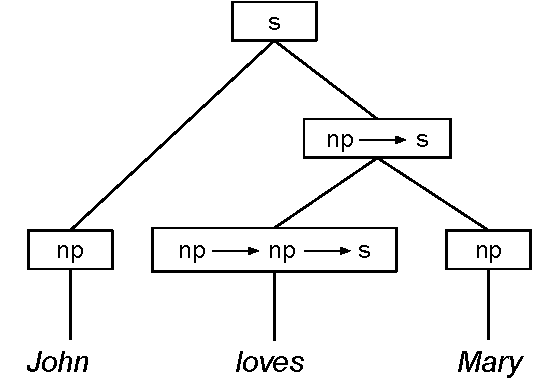
\includegraphics[width=0.4\textwidth]{images/JohnLovesMary.pdf}
\caption{Syntactic parse tree of sentence \txt{John loves Mary}.} \label{fig:JohnLovesMary-2}
\end{figure}
\begin{align}
\D = \ & \I{loves} \I{Mary} \I{John}  \notag \\
= \ & (\lambda \Y2 \X2. \X2( \lambda \x1. \Y2 (\lambda \y1. ( \lambda e' \phi. \textbf{love} \x1 \y1 \land \phi e' ))) )  \I{Mary} \I{John}  \notag \\
\bconv \ & (\lambda  \X2. \X2( \lambda \x1. \I{Mary}  (\lambda \y1. ( \lambda e' \phi. \textbf{love} \x1 \y1 \land \phi e' ))) )  \I{John}  \notag \\
\bconv \ &    \I{John}( \lambda \x1. \I{Mary}  (\lambda \y1. ( \lambda e' \phi. \textbf{love} \x1 \y1 \land \phi e' )))   \notag \\
= \ &    \I{John}( \lambda \x1. (\lambda \P2. \lambda e \phi. \P2 \textbf{m} e (\lambda e. \phi (\upii{\textbf{m}}{e'})))  (\lambda \y1. ( \lambda e' \phi. \textbf{love} \x1 \y1 \land \phi e' )))   \notag \\
\bconv \ &    \I{John}( \lambda \x1.  \lambda e \phi. (\lambda \y1. ( \lambda e' \phi. \textbf{love} \x1 \y1 \land \phi e' )) \textbf{m} e (\lambda e'. \phi (\upii{\textbf{m}}{e'})))   \notag \\
\bconv \ &    \I{John}( \lambda \x1.  \lambda e \phi. ( \lambda e' \phi. \textbf{love} \x1 \textbf{m} \land \phi e' ) e (\lambda e' . \phi (\upii{\textbf{m}}{e'})))   \notag \\
\bred \ &    \I{John}( \lambda \x1.  \lambda e \phi.  \textbf{love} \x1 \textbf{m} \land  (\lambda e' .\phi (\upii{\textbf{m}}{e'}) e))   \notag \\
\bconv \ &    \I{John}( \lambda \x1.  \lambda e \phi.  \textbf{love} \x1 \textbf{m} \land  \phi (\upii{\textbf{m}}{e} ))   \notag \\
= \ &    ( \lambda \P2. \lambda e \phi. \P2 \textbf{j} e (\lambda e' .\phi (\upii{\textbf{j}}{e'})))( \lambda \x1.  \lambda e \phi.  \textbf{love} \x1 \textbf{m} \land  \phi (\upii{\textbf{m}}{e} ))   \notag \\
\bconv \ &    \lambda e \phi. ( \lambda \x1.  \lambda e \phi.  \textbf{love} \x1 \textbf{m} \land  \phi (\upii{\textbf{m}}{e} ))   \textbf{j} e (\lambda e' . \phi (\upii{\textbf{j}}{e'})) \notag \\
\bred \ &    \lambda e \phi.  \textbf{love}  \textbf{j} \textbf{m} \land   (\lambda e' .\phi (\upii{\textbf{j}}{e'})) (\upii{\textbf{m}}{e} )  \notag \\
\bconv \ &    \lambda e \phi.  \textbf{love}  \textbf{j} \textbf{m} \land   \phi (\upii{\textbf{j}}{\upii{\textbf{m}}{e} })   \label{eq:2006:JohnLovesMary} 
\end{align}
\end{example}

To cope with anaphora, the context has to be accessed. This is accomplished by a special function $\sel$ of type $(\gamma \rightarrow \iota)$ that takes a context and returns an individual. The function $\sel$ is assumed to implement an anaphora resolution algorithm and to work as an oracle always retrieving the correct antecedent. This allows to interpret pronouns as shown, for example, for \txt{he} below:
\begin{align}
\I{he} =  \overbrace{\lambda \P2^{^\iota \rightarrow \gamma \rightarrow (\gamma \rightarrow o) \rightarrow o}. \lambda e^{\gamma} \phi^{\gamma \rightarrow o}. \overbrace{\overbrace{\overbrace{\P2 ( \overbrace{\sel_{he} e}^{\iota} )}^{\gamma \rightarrow (\gamma \rightarrow o) \rightarrow o} e}^{ (\gamma \rightarrow o) \rightarrow o} \ \phi }^{o}}^{(\iota \rightarrow \gamma \rightarrow (\gamma \rightarrow o) \rightarrow o) \rightarrow \gamma \rightarrow (\gamma \rightarrow o) \rightarrow o}  \label{eq:he:2006}
%\I{he} = \lambda \P2. \lambda e \phi. \P2 (\sel_{he}e)e\phi
\end{align}

\begin{example}[$\S$, \txt{He smiles at her}] \label{ex:2006:HeSmilesAtHer} The meaning of the sentence~\eqref{HeSmilesAtHer-2006} computed in accordance with the parse-tree shown in Figure~\ref{fig:ptS3-2006}  is as follows:
\enumsentence{\txt{He smiles at her.} \label{HeSmilesAtHer-2006}}
\begin{align}
\S = \ & \I{smiles\_at} \I{her} \I{he} \notag \\
 = \ & (\lambda \Y2 \X2. \X2( \lambda \x1. \Y2 (\lambda \y1. ( \lambda e' \phi. \textbf{smile} \x1 \y1 \land \phi e' ))) )  \I{her} \I{he} \notag \\
\bconv \ & (\lambda  \X2. \X2( \lambda \x1.  \I{her}  (\lambda \y1. ( \lambda e' \phi. \textbf{smile} \x1 \y1 \land \phi e' ))) ) \I{he} \notag \\
\bconv \ &   \I{he} ( \lambda \x1.  \I{her}  (\lambda \y1. ( \lambda e' \phi. \textbf{smile} \x1 \y1 \land \phi e' ))) \notag  \\
= \ &   \I{he} ( \lambda \x1.  (\lambda \P2. \lambda e \phi. \P2 (\sel_{her}e)e\phi)  (\lambda \y1. ( \lambda e' \phi. \textbf{smile} \x1 \y1 \land \phi e' ))) \notag \\
 \bconv \ &   \I{he} ( \lambda \x1.  (\lambda e \phi.  (\lambda \y1. ( \lambda e' \phi. \textbf{smile} \x1 \y1 \land \phi e' )) (\sel_{her}e)e\phi) ) \notag \\
  \bconv \ &   \I{he} ( \lambda \x1.  (\lambda e \phi.   ( \lambda e' \phi. \textbf{smile} \x1  (\sel_{her}e) \land \phi e' ) e\phi) ) \notag \\
 \bred \ &   \I{he} ( \lambda \x1.  (\lambda e \phi.  \textbf{smile} \x1  (\sel_{her}e) \land \phi e) ) \notag \\
  = \ &  (\lambda \P2. \lambda e \phi. \P2 (\sel_{he}e)e\phi) ( \lambda \x1.  (\lambda e \phi.  \textbf{smile} \x1  (\sel_{her}e) \land \phi e) ) \notag \\
\bconv \ & \lambda e \phi. ( \lambda \x1.  (\lambda e \phi.  \textbf{smile} \x1  (\sel_{her}e) \land \phi e) )  (\sel_{he}e)e\phi \notag \\
\bconv \ & \lambda e \phi.   (\lambda e \phi.  \textbf{smile}  (\sel_{he}e)  (\sel_{her}e) \land \phi e) e\phi \notag \\
\bred \ & \lambda e \phi.   \textbf{smile}  (\sel_{he}e)  (\sel_{her}e) \land \phi e \label{eq:2006:HeSmilesAtHer}
\end{align}
\end{example}

\begin{figure}[h]
 \centering
    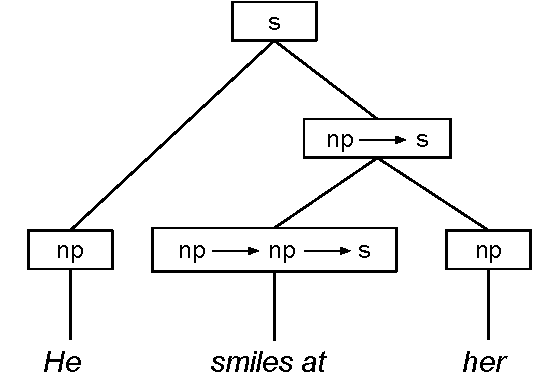
\includegraphics[width=0.4\textwidth]{images/HeSmilesatHer.pdf}
\caption{Syntactic parse tree of sentence \txt{He smiles at her}.} \label{fig:ptS3-2006}
\end{figure}

As Example~\ref{ex:2006:HeSmilesAtHer} shows, Sentence~\eqref{HeSmilesAtHer-2006} is meaningful in de~Groote's approach in the sense that it has an interpretation~\eqref{eq:2006:HeSmilesAtHer}. However, the function $\sel$ can return individuals for \txt{he} and \txt{her} only when the sentence is evaluated over some context containing the corresponding antecedents. This can be done when the sentence is uttered in a discourse and the representation of this discourse is already computed. When the meaning of the discourse is updated with the meaning of the sentence, the pronominal anaphora is resolved. 

Discourses in~\cite{deGroote:2006:Towards-a-Montagovian-Account-of-Dynamics} are, like sentences, interpreted as terms of type $(\gamma \rightarrow (\gamma \rightarrow o) \rightarrow o)$.  The update of a discourse interpreted as $\D$ with a sentence interpreted as $\S$ results in interpretation $\updt \ \D \ \S$ of a new discourse. This interpretation is defined by the following equation:
\begin{align}
\updt \ \D \ \S \defeq \overbrace{\lambda e^{\gamma} \phi^{\gamma \rightarrow o}. \overbrace{ \overbrace{\D^{\gamma \rightarrow (\gamma \rightarrow o) \rightarrow o}  e}^{(\gamma \rightarrow o) \rightarrow o} (\overbrace{\lambda e'^{\gamma}. \overbrace{\overbrace{\S^{\gamma \rightarrow (\gamma \rightarrow o) \rightarrow o}  e'}^{ (\gamma \rightarrow o) \rightarrow o} \phi}^{o}}^{\gamma \rightarrow o})}^{o}}^{\gamma \rightarrow (\gamma \rightarrow o) \rightarrow o} \label{eq:updtDS:2006}
\end{align}

\begin{example}[$\updt \ \D \ \S$]
Now interpretations~\eqref{eq:2006:JohnLovesMary} and~\eqref{eq:2006:HeSmilesAtHer} can be composed through equation~\eqref{eq:updtDS:2006}, regarding~\eqref{sent:JlovesM-2006} as the discourse updated with the sentence~\eqref{HeSmilesAtHer-2006}. This leads to the interpretation of the piece of discourse~\eqref{sen:JLMHeSH:2006}:
\enumsentence{\txt{John loves Mary. He smiles at her.} \label{sen:JLMHeSH:2006}}
\begin{align}
& \lambda e \phi. (\overbrace{\lambda e \phi.  \textbf{love}  \textbf{j} \textbf{m} \land   \phi (\upii{\textbf{j}}{\upii{\textbf{m}}{e} }) }^{\D}  ) e (\lambda e'. (\overbrace{\lambda e \phi.   \textbf{smile}  (\sel_{he}e)  (\sel_{her}e) \land \phi e}^{\S}) e' \phi ) \notag \\
\bred \ & \lambda e \phi. (\lambda e \phi.  \textbf{love}  \textbf{j} \textbf{m} \land   \phi (\upii{\textbf{j}}{\upii{\textbf{m}}{e} }) ) e (\lambda e'.  \textbf{smile}  (\sel_{he}e')  (\sel_{her}e') \land \phi e' ) \notag \\
\bred \ & \lambda e \phi.\textbf{love}  \textbf{j} \textbf{m} \land    (\lambda e'.  \textbf{smile}  (\sel_{he}e')  (\sel_{her}e') \land \phi e' )  (\upii{\textbf{j}}{\upii{\textbf{m}}{e} }) \notag \\
\bconv \ & \lambda e \phi.\textbf{love}  \textbf{j} \textbf{m} \land    \textbf{smile}  (\sel_{he}(\upii{\textbf{j}}{\upii{\textbf{m}}{e} }))  (\sel_{her}(\upii{\textbf{j}}{\upii{\textbf{m}}{e} })) \land \phi  (\upii{\textbf{j}}{\upii{\textbf{m}}{e} }) \label{int:JLMHeSH:2006}
\end{align}
\end{example}

Interpretation~\eqref{int:JLMHeSH:2006} of the discourse consisting of the utterance of~\eqref{sen:JLMHeSH:2006} is computed in a compositional manner. Note that the context of the interpretation of the first sentence is passed to $\sel$ operators of the interpretation of the second sentence. Assuming that an anaphora resolution mechanism is implemented in $\sel$, the following semantic representation of~\eqref{sen:JLMHeSH:2006} is obtained: 
\begin{align}
\lambda e \phi.\textbf{love} \  \textbf{j} \ \textbf{m} \land    \textbf{smile}  \ \textbf{j} \ \textbf{m} \land \phi  (\upii{\textbf{j}}{\upii{\textbf{m}}{e} }) \label{int:JLMHeSH:2006-2}
\end{align}
The context $(\upii{\textbf{j}}{\upii{\textbf{m}}{e} })$ in~\eqref{int:JLMHeSH:2006} (and hence in~\eqref{int:JLMHeSH:2006-2})  is accessible for future computation. This means that the individuals $\textbf{j}$ and $\textbf{m}$ can serve as ancestors for anaphoric pronouns in the following sentences. However, this is not always the case. For example, assuming accessibility constraint requirements of DRT, the individuals introduced by quantifiers in Sentence~\eqref{donkey-every-2006} should not be accessible for anaphoric triggers outside of the sentence. However, they clearly should be accessible for anaphoric pronouns within the sentence. 
\enumsentence{ \txt{Every farmer who owns a donkey beats it.} \label{donkey-every-2006}}
This accessibility constraint can also be implemented in de~Groote's approach. For example, lexical items of~\eqref{donkey-every-2006} can be assigned meanings shown in Table~\ref{tbl:donkey-lexical-2006} that lead to the desirable interpretation of the sentence, as demonstrated below. Since the lexical interpretations are dynamic, the resulting dynamic meaning of the donkey sentence does not suffer the drawbacks of the static meaning.

\begin{table}
\begin{footnotesize}
\begin{tabular}{ l l l l l }
  Lexical item & Syntactic category  & Continuation-based interpretation in {\G}\\
  \hline
  \\
  \txt{farmer} & n & $\lambda \x1 e \phi.  \cfarmer \x1 \land \phi e  $  \\
  \txt{donkey} & n & $\lambda \x1 e \phi.  \cdonkey \x1  \land \phi e  $  \\
   \txt{owns} & np $\rightarrow$ np $\rightarrow$ s & $ \lambda \Y2 \X2. \X2 ( \lambda \x1. \Y2 (\lambda \y1. ( \lambda e' \phi. \cown \x1 \y1 \land \phi e'))) $ \\
 \txt{beats} & np $\rightarrow$ np $\rightarrow$ s  & $ \lambda \Y2 \X2. \X2 ( \lambda \x1. \Y2 (\lambda \y1. ( \lambda e' \phi. \cbeat \x1 \y1 \land \phi e'))) $ \\
    \txt{a} &  n $\rightarrow$ np & $ \lambda \P2 \Q2. \lambda e \phi. \exists (\lambda \x1. \P2  \x1 e ( \lambda e'. \Q2 \x1  (\upii{\x1}{e'}) \phi ) ) $ \\
    \txt{every} & n $\rightarrow$ np & $ \lambda \P2 \Q2. \lambda e \phi. (\forall \x1. \neg (\P2 \x1 e (\lambda e'. \neg (\Q2 \x1 (\upii{\x1}{e'})  (\lambda e'''. \top)  ))))  \land \phi e$ \\
   \txt{who} & (np~$\rightarrow$~s)~$\rightarrow$~n~$\rightarrow$~n & $\lambda \R2 \Q2 \x1. \lambda e \phi. \Q2 \x1 e (\lambda e'. \R2 (\lambda \P2. \P2 \x1) e' \phi)$ \\
   \txt{it} & np & $ \lambda \P2. \lambda e \phi. \P2 ( \sel_{it} e) e \phi  $  
   \end{tabular}
\caption{Continuation-based interpretations of lexical items of the sentence \txt{Every farmer who owns a donkey beats it} in framework {\G}.} \label{tbl:donkey-lexical-2006}
\end{footnotesize}
\end{table}


\begin{example}[\txt{Every farmer who owns a donkey beats it}]
The meaning of the noun phrase \txt{a donkey} is computed by reducing the term $\trr{\I{a}} \trr{\I{donkey}} $:
\begin{align}
 \trr{\I{a}} \trr{\I{donkey}} 
 = \  & ( \lambda \P2 \Q2. \lambda e \phi. \exists (\lambda \y1. \P2  \y1 e ( \lambda e'. \Q2 \y1  (\upii{\y1}{e'}) \phi ) ) ) \trr{\I{donkey}} \notag \\ 
\bconv \ &  \lambda  \Q2. \lambda e \phi. \exists (\lambda \y1. \trr{\I{donkey}}  \y1 e ( \lambda e'. \Q2 \y1  (\upii{\y1}{e'}) \phi ) )  \notag \\ 
= \ &   \lambda  \Q2. \lambda e \phi. \exists (\lambda \y1. (\lambda \x1 e \phi.  \cdonkey \x1  \land \phi e )  \y1 e ( \lambda e'. \Q2 \y1  (\upii{\y1}{e'}) \phi ) )  \notag \\ 
\bconv \ & \lambda  \Q2. \lambda e \phi. \exists (\lambda \y1. (\lambda  e \phi.  \cdonkey \y1  \land \phi e )   e ( \lambda e'. \Q2 \y1  (\upii{\y1}{e'}) \phi ) )  \notag \\ 
\bred \  & \lambda  \Q2. \lambda e \phi. \exists (\lambda \y1.  \cdonkey \y1  \land  ( \lambda e'. \Q2 \y1  (\upii{\y1}{e'}) \phi ) e )  \notag \\ 
\bconv \  &  \lambda  \Q2. \lambda e \phi. \exists (\lambda \y1.  \cdonkey \y1  \land  \Q2 \y1  (\upii{\y1}{e}) \phi )  \label{eq:adonkey-nf-computed-2006}
\end{align}
Note that in Equation~\eqref{eq:adonkey-nf-computed-2006} the environment passed as an argument to $\Q2$ contains the variable $\y1$ introduced by the existential quantifier. This means that this variable is available to the formula $\Q2$. 
Note also that the continuation $\phi$ of the term~\eqref{eq:adonkey-nf-computed-2006}  is within the scope of the existential quantifier. 

The meaning of the verb phrase \txt{owns a donkey} is computed by $\beta$-reducing the term $  \trr{\I{owns}}  (\trr{\I{a}} \trr{\I{donkey}} )  $:
\begin{align*}
& \trr{\I{owns}}  (\trr{\I{a}} \trr{\I{donkey}} ) \\
= \ & ( \lambda \Y2 \X2. \X2 ( \lambda \x1. \Y2 (\lambda \y1. ( \lambda e' \phi. \cown \x1 \y1 \land \phi e'))) ) (\trr{\I{a}} \trr{\I{donkey} } )  \\
\bconv \ &  \lambda  \X2. \X2 ( \lambda \x1. (\trr{\I{a}} \trr{\I{donkey} } )  (\lambda \y2. ( \lambda e' \phi. \cown \x1 \y1 \land \phi e')))  \\
= \ & \lambda  \X2. \X2 ( \lambda \x1. ( \lambda  \Q2. \lambda e \phi. \exists (\lambda \y1.  \cdonkey \y1  \land  \Q2 \y1  (\upii{\y1}{e}) \phi )  )  (\lambda \y1. ( \lambda e' \phi. \cown \x1 \y1 \land \phi e')))  \\
\bconv \ &   \lambda  \X2. \X2 ( \lambda \x1. ( \lambda e \phi. \exists (\lambda \y1.  \cdonkey \y1  \land  (\lambda \y1. ( \lambda e' \phi. \cown \x1 \y1 \land \phi e')) \y1  (\upii{\y1}{e}) \phi )  )  )  \\
\bred \ &    \lambda  \X2. \X2 ( \lambda \x1. ( \lambda e \phi. \exists (\lambda \y1.  \cdonkey \y1  \land  \cown \x1 \y1 \land \phi (\upii{\y1}{e}) )  )  )  
\end{align*}
The dynamic meaning of the relative clause \txt{who owns a donkey} is computed as follows:
\begin{align}
& \trr{\I{who}}  (\trr{\I{owns}}  (\trr{\I{a}} \trr{\I{donkey}} )) \notag \\
= \ &  (\lambda \R2 \Q2 \x1. \lambda e \phi. \Q2 \x1 e (\lambda e'. \R2 (\lambda \P2. \P2 \x1) e' \phi)) (\trr{\I{owns}}  (\trr{\I{a}}  \trr{\I{donkey}} )) \notag \\
\bconv \ &  \lambda  \Q2 \x1. \lambda e \phi. \Q2 \x1 e (\lambda e'. (\trr{\I{owns}}  (\trr{\I{a}} \ \trr{\I{donkey}} ))  (\lambda \P2. \P2 \x1) e' \phi) \notag \\
= \ &   \lambda  \Q2 \x1. \lambda e \phi. \Q2 \x1 e (\lambda e'. (   \lambda  \X2. \X2 ( \lambda \x1. ( \lambda e \phi. \exists (\lambda \y1.  \cdonkey \y1  \land  \cown \x1 \y1 \land \phi (\upii{\y1}{e}) )  )  )  )  (\lambda \P2. \P2 \x1) e' \phi) \notag \\
\bconv \ &  \lambda  \Q2 \x1. \lambda e \phi. \Q2 \x1 e (\lambda e'.  (\lambda \P2. \P2 \x1) ( \lambda \x1. ( \lambda e \phi. \exists (\lambda \y1.  \cdonkey \y1  \land  \cown \x1 \y1 \land \phi (\upii{\y1}{e}) )  )  )    e' \phi) \notag \\
\bconv \ &  \lambda  \Q2 \x1. \lambda e \phi. \Q2 \x1 e (\lambda e'.   ( \lambda \x1. ( \lambda e \phi. \exists (\lambda \y1.  \cdonkey \y1  \land  \cown \x1 \y1 \land \phi (\upii{\y1}{e}) )  )  ) \x1    e' \phi) \notag \\
\bconv \ &  \lambda  \Q2 \x1. \lambda e \phi. \Q2 \x1 e (\lambda e'.  ( \lambda e \phi. \exists (\lambda \y1.  \cdonkey \y1  \land  \cown \x1 \y1 \land \phi (\upii{\y1}{e}) )  )     e' \phi) \notag \\
\bred \ &  \lambda  \Q2 \x1. \lambda e \phi. \Q2 \x1 e (\lambda e'.  \exists (\lambda \y1.  \cdonkey \y1  \land  \cown \x1 \y1 \land \phi (\upii{\y1}{e'}) )  )    \label{eq:whoownsadonkey-nf-2006}
\end{align}
The meaning of \txt{farmer who owns a donkey} is computed by applying the $\lambda$-term~\eqref{eq:whoownsadonkey-nf-2006} to the lexical interpretation of \txt{farmer}:
\begin{align*}
& (\trr{\I{who}}  (\trr{\I{owns}}  (\trr{\I{a}}  \trr{\I{donkey}} ) ) )\trr{\I{farmer}} \\
 = \ &  (  \lambda  \Q2 \x1. \lambda e \phi. \Q2 \x1 e (\lambda e'.  \exists (\lambda \y1.  \cdonkey \y1  \land  \cown \x1 \y1 \land \phi (\upii{\y1}{e'}) )  ) ) \trr{\I{farmer}}  \\
 \bconv \ &   \lambda   \x1. \lambda e \phi.  \trr{\I{farmer}}  \x1 e (\lambda e'.  \exists (\lambda \y1.  \cdonkey \y1  \land  \cown \x1 \y1 \land \phi (\upii{\y1}{e'}) )  ) \\
 = \ &    \lambda   \x1. \lambda e \phi.  (\lambda \x1 e \phi.  \cfarmer \x1 \land \phi e) \x1 e (\lambda e'.  \exists (\lambda \y1.  \cdonkey \y1  \land  \cown \x1 \y1 \land \phi (\upii{\y1}{e'}) )  ) \\
\bconv \ & \lambda   \x1. \lambda e \phi.  (\lambda  e \phi.  \cfarmer \x1 \land \phi e)  e (\lambda e'.  \exists (\lambda \y1.  \cdonkey \y1  \land  \cown \x1 \y1 \land \phi (\upii{\y1}{e'}) )  ) \\
\bred \ & \lambda   \x1. \lambda e \phi. \cfarmer \x1 \land  (\lambda e'.  \exists (\lambda \y1.  \cdonkey \y1  \land  \cown \x1 \y1 \land \phi (\upii{\y1}{e'}) )  ) e   \\
\bconv \ &  \lambda   \x1. \lambda e \phi. \cfarmer \x1 \land   \exists (\lambda \y1.  \cdonkey \y1  \land  \cown \x1 \y1 \land \phi (\upii{\y1}{e}) )         
\end{align*}
The dynamic meaning of the noun phrase \txt{every farmer who owns a donkey} is computed by applying the meaning of \txt{every} to the meaning of \txt{farmer who owns a donkey}.  
%\begin{footnotesize}
\begin{align}
& \trr{\I{every}}  ((\trr{\I{who}}  (\trr{\I{owns}}  (\trr{\I{a}}  \trr{\I{donkey}} ) )) \trr{\I{farmer}}  )  \notag \\
= \ & ( \lambda \P2 \Q2. \lambda e \phi. (\forall \x1. \neg (\P2 \x1 e (\lambda e'. \neg (\Q2 \x1 (\upii{\x1}{e'})  (\lambda e'''. \top)  ))))  \land \phi e) \notag \\
&  ((\trr{\I{who}}  (\trr{\I{owns}}  (\trr{\I{a}} \ \trr{\I{donkey}} ) )) \trr{\I{farmer}}  )   \notag \\
\bconv \ &   \lambda  \Q2. \lambda e \phi. (\forall \x1. \neg ( ((\trr{\I{who}}  (\trr{\I{owns}}  (\trr{\I{a}} \ \trr{\I{donkey}} ) )) \trr{\I{farmer}}  ) \notag \\
& \phantom{\lambda  \Q2. \lambda e \phi. (\forall \x1. \neg (} \x1 e (\lambda e'. \neg (\Q2 \x1 (\upii{\x1}{e'})  (\lambda e'''. \top)  ))))  \land \phi e  \notag \\
= \ &    \lambda  \Q2. \lambda e \phi. (\forall \x1. \neg ( (  \lambda   \x1. \lambda e \phi. \cfarmer \x1 \land   \exists (\lambda \y1.  \cdonkey \y1  \land  \cown \x1 \y1 \land \phi (\upii{\y1}{e}) )  )  \notag  \\
& \phantom{\lambda  \Q2. \lambda e \phi. (\forall \x1. \neg (} \x1 e (\lambda e'. \neg (\Q2 \x1 (\upii{\x1}{e'})  (\lambda e'''. \top)  ))))  \land \phi e  \notag \\
\bconv \ &     \lambda  \Q2. \lambda e \phi. (\forall \x1. \neg ( (  \lambda e \phi. \cfarmer \x1 \land   \exists (\lambda \y1.  \cdonkey \y1  \land  \cown \x1 \y1 \land \phi (\upii{\y1}{e}) )  )  \notag \\
& \phantom{\lambda  \Q2. \lambda e \phi. (\forall \x1. \neg (} e (\lambda e'. \neg (\Q2 \x1 (\upii{\x1}{e'})  (\lambda e'''. \top)  ))))  \land \phi e  \notag \\
\bred \ &   \lambda  \Q2. \lambda e \phi. (\forall \x1. \neg ( \cfarmer \x1 \land   \exists (\lambda \y1.  \cdonkey \y1  \land  \cown \x1 \y1 \land  \notag \\
& \phantom{\lambda  \Q2. \lambda e \phi. (\forall \x1. \neg ( \cfarmer \x1 \land   \exists (\lambda \y1.  \cdonkey \y1  \land  \cown}
(\lambda e'. \neg (\Q2 \x1 (\upii{\x1}{e'})  (\lambda e'''. \top)  )) (\upii{\y1}{e}) ) ))  \land \phi e  \notag \\
\bconv \ &   \lambda  \Q2. \lambda e \phi. (\forall \x1. \neg ( \cfarmer \x1 \land   \exists (\lambda \y1.  \cdonkey \y1  \land  \cown \x1 \y1 \land  \neg (\Q2 \x1 (\upii{\x1}{\upii{\y1}{e}})  (\lambda e'''. \top)  ) ) ))  \land \phi e  \label{eq:everyfarmerwhoownsadonkey-nf-2006}
\end{align}


Note that in Equation~\eqref{eq:everyfarmerwhoownsadonkey-nf-2006} the environment containing all the individuals with their properties collected during the computation is locally passed to the formula $\Q2$. The continuation $\phi$ receives only the environment $e$ that is passed to the term as an argument; therefore, all individuals collected during the computation of the meaning of \txt{every farmer who owns a donkey} are not available outside the logical formula interpreting this phrase.

The meaning of the verb phrase \txt{beats it} is computed as follows:
\begin{align}
 \trr{\I{beats}}  \trr{\I{it}}  
 = \ &  (\lambda \Y2 \X2. \X2 ( \lambda \x1. \Y2 (\lambda \y1. ( \lambda e' \phi. \cbeat \x1 \y1 \land \phi e')))) \trr{\I{it}}   \notag \\
 \bconv \ & \lambda  \X2. \X2 ( \lambda \x1. \trr{\I{it}}  (\lambda \y1. ( \lambda e' \phi. \cbeat \x1 \y1 \land \phi e')))   \notag \\
 = \ & \lambda  \X2. \X2 ( \lambda \x1. (  \lambda \P2. \lambda e \phi. \P2 ( \sel_{it} e) e \phi )  (\lambda \y1. ( \lambda e' \phi. \cbeat \x1 \y1 \land \phi e')))   \notag \\
 \bconv \ & \lambda  \X2. \X2 ( \lambda \x1. \lambda e \phi. (\lambda \y1. ( \lambda e' \phi. \cbeat \x1 \y1 \land \phi e')) ( \sel_{it} e) e \phi )    \notag \\
 \bconv \ &  \lambda  \X2. \X2 ( \lambda \x1. \lambda e \phi.  ( \lambda e' \phi. \cbeat \x1  ( \sel_{it} e)  \land \phi e') e \phi )    \notag \\
  \bred \ &  \lambda  \X2. \X2 ( \lambda \x1. \lambda e \phi.   \cbeat \x1  ( \sel_{it} e)  \land \phi e )  \label{eq:beatsit-nf-2006}
\end{align}
Finally, the dynamic meaning of the sentence is computed by applying the \\ term~\eqref{eq:beatsit-nf-2006} to the term~\eqref{eq:everyfarmerwhoownsadonkey-nf-2006}:
\begin{align}
& \trr{\I{beats}}  \trr{\I{it}} (\trr{\I{every}}  ((\trr{\I{who}}  (\trr{\I{owns}}  (\trr{\I{a}}  \trr{\I{donkey}} ) ) ) \trr{\I{farmer}}  )) \notag \\
= \ & ( \lambda  \X2. \X2 ( \lambda \x1. \lambda e \phi.   \cbeat \x1  ( \sel_{it} e)  \land \phi e )) \notag \\
&  (\trr{\I{every}}  ((\trr{\I{who}}  (\trr{\I{owns}}  (\trr{\I{a}}  \trr{\I{donkey}} ) ) ) \trr{\I{farmer}}  )) \notag \\
\bconv \ &   (\trr{\I{every}}  ((\trr{\I{who}}  (\trr{\I{owns}}  (\trr{\I{a}}  \trr{\I{donkey}} ) ) ) \trr{\I{farmer}}  ))  ( \lambda \x1. \lambda e \phi.   \cbeat \x1  ( \sel_{it} e)  \land \phi e ) \notag \\
= \ &    ( \lambda  \Q2. \lambda e \phi. (\forall \x1. \neg ( \cfarmer \x1 \land   \exists (\lambda \y1.  \cdonkey \y1  \land  \cown \x1 \y1 \land  \neg (\Q2 \x1 (\upii{\x1}{\upii{\y1}{e}})  (\lambda e'''. \top)  ) ) ))  \land \phi e ) \notag \\
&  ( \lambda \x1. \lambda e \phi.   \cbeat \x1  ( \sel_{it} e)  \land \phi e ) \notag \\
\bconv \ &    \lambda e \phi. (\forall \x1. \neg ( \cfarmer \x1 \land   \exists (\lambda \y1.  \cdonkey \y1  \land  \cown \x1 \y1 \land \notag \\
& \phantom{aaaaaaaaaa}  \neg (( \lambda \x1. \lambda e \phi.   \cbeat \x1  ( \sel_{it} e)  \land \phi e ) \x1 (\upii{\x1}{\upii{\y1}{e}})  (\lambda e'''. \top)  ) ) ))  \land \phi e    \notag \\
\bconv \ &  \lambda e \phi. (\forall \x1. \neg ( \cfarmer \x1 \land   \exists (\lambda \y1.  \cdonkey \y1  \land  \cown \x1 \y1 \land \notag \\
& \phantom{aaaaaaa} \neg (( \lambda e \phi.   \cbeat \x1  ( \sel_{it} e)  \land \phi e ) (\upii{\x1}{\upii{\y1}{e}})  (\lambda e'''. \top)  ) ) ))  \land \phi e    \notag \\
\bred \ &  \lambda e \phi. (\forall \x1. \neg ( \cfarmer \x1 \land   \exists (\lambda \y1.  \cdonkey \y1  \land  \cown \x1 \y1 \land \notag \\
& \phantom{aaaaaaa} \neg (  \cbeat \x1  ( \sel_{it}  (\upii{\x1}{\upii{\y1}{e}}))  \land (\lambda e'''. \top)  (\upii{\x1}{\upii{\y1}{e}})   ) ) ))  \land \phi e    \notag \\
\bconv \ &\lambda e \phi. (\forall \x1. \neg ( \cfarmer \x1 \land   \exists (\lambda \y1.  \cdonkey \y1  \land  \cown \x1 \y1 \land  \neg (  \cbeat \x1  ( \sel_{it}  (\upii{\x1}{\upii{\y1}{e}}))  \land  \top  ) ) ))  \land \phi e     \label{eq:donkey-nf-meaning-2006}
\end{align}

The resulting dynamic interpretation~\eqref{eq:donkey-nf-meaning-2006} of the donkey sentence is logically equivalent to~\eqref{eq:donkey-nf-meaning-2-2006}:
\begin{align}
 \lambda e \phi. \forall ( \lambda \x1.  \cfarmer \x1  \rightarrow    \forall ( \lambda \y1.  ( \cdonkey \y1 \land  \cown \x1 \y1 ) \rightarrow   \cbeat \x1  ( \sel_{it} (\y1 :: \x1 :: e))  )  ) )  \land \phi e  \label{eq:donkey-nf-meaning-2-2006}
\end{align}
Note that, in accordance with DRT's accessibility constraint, the individuals bound by quantifiers are not accessible outside the sentence. 
\end{example}

%The dynamic formula~\eqref{eq:donkey-nf-meaning-2-2006}, computed using the dynamic lexical interpretations, does not have the drawbacks of the static formula~\eqref{eq:donkey-st-meaning}, computed using the static lexical interpretations. 

First of all, the second argument of $\cbeat$, standing for the anaphoric pronoun, is not a free dummy variable, but a term $( \sel_{it} (\y1 :: \x1 :: e))$. This term consists of the selection function $\sel$ that takes as argument a context containing the available individuals ``collected'' during the computation. Thus, in contrast to the static case, the second argument of $\cbeat$ is self-sufficient: the function $\sel$, which implements an anaphora resolution algorithm, selects a required individual from the context. In the current case, the selection function returns the individual $\y1$, leading to the final dynamic meaning~\eqref{eq:donkey-nf-meaning-3-2006} of Sentence~\eqref{donkey-every-2006}:
\begin{align}
\lambda e \phi. \forall ( \lambda \x1.  \cfarmer \x1  \rightarrow    \forall ( \lambda \y1.  ( \cdonkey \y1 \land  \cown \x1 \y1 ) \rightarrow   \cbeat \x1 \y1  ) )  \land \phi e  \label{eq:donkey-nf-meaning-3-2006}
\end{align}

Moreover, in the dynamic interpretation, unlike in the static one, the formula $\cbeat \x1 \y1 $ is within the scope of the quantifier binding the variable $y$, exactly as desired.  Furthermore, the quantifier binding $y$ has been changed during the computation from existential to universal, which is also impossible in the static approach. These improvements are the consequences of employing a continuation-passing technique. 

The list below summarizes the advantages that de~Groote's approach brought to compositional semantics:

\begin{itemize}

\item The approach is independent of the intermediate language\footnote{See Section~\ref{sec:MS}.} used to express meanings of the expressions. This allows to use mathematical and logical theories developed outside computational linguistics.\footnote{An extension of first logic language with $\lambda$ is used here because it is convenient and intuitive.} Therefore, natural language phenomena can be explained in terms of well-established and well-understood theories.

\item Variables do not have any special status and are variables in the usual mathematical sense. Therefore, the notions of free and bound variables are standard.  

\item There is no imperative dynamic notions as assignment functions, therefore destructive assignment problem does not hold. Meanings assigned to expressions are closed $\lambda$-terms. 

\item There is no need for rules that artificially extend the scope of quantifiers.

\item Context and content are regarded separately, but they do interact during the computation of the meaning of discourse.  

\item The approach does not depend on any specific structure given to the context. In contrast, context is defined as a term of type parameter $\gamma$ and, therefore, its structure can be altered when necessary.

\item The approach is truly compositional: the meaning of a complex expression is computed by $\beta$-reducing the composition of the meanings of its lexical items.

\end{itemize}


\section{Comparison With Other Work}

\cite{GroenendijkStokhof:1991:Dynamic-Predicate-Logic}

\section{Higher Order Case}


\section{Higher order case and Conservation}


This is a test. This is another test. Yes indeed.


\bibliographystyle{abbrv}
\bibliography{bibliography}

\end{document}
